\section{Ablations}
\label{sec:ablations}
% \tianyu{split into subsections; refer back to the main body; can refer to subsection, copy the title of the paragraph; }

% \tianyu{avoid putting figures too far away. Add links back to the texts in captions.}

\subsection{Experimental details}\label{appsec:experiment-detail}
We provide more details for experiments in Section \ref{sec:bb_task}. We train transformers with positional embedding, pre-layer norm, $\softmax$ activation in \attn, and ReLU activation in \mlp. 
We use Adam with constant learning rate $0.0003$, $\beta_1=0.9$, $\beta_2=0.99$, $\eps=10^{-8}$, and a weight decay of $0.01$. We choose a learning rate of $0.03$ for the SGD. In each training step, we resample from the BB task with a batch size of $B=512$ and sequence length $N=256$. Unless otherwise specified, the model is trained for $10,000$ steps. Results are consistent across different random seeds.

\subsection{Additional attention plots of a 1-layer transformer trained on the BB task}
\label{appsec:additional-attn-maps}
We provide more attention plots of the 1-layer transformer on sequences other than those shown in Figure~\ref{fig:bbm-attn}.
Figure~\ref{appfigure:more-attn} presents more attention-weight heat maps of the one-layer transformer model trained on the BB task. All attention maps show the attention sink phenomenon. Some non-trigger tokens present attention patterns other than attention sink. For example, trigger tokens serve as attention sinks in some inputs in Figure~\ref{appfig:trigger-sink}.
\begin{figure}[h]
  \centering
  \begin{minipage}{0.3\textwidth}
      \centering
      \subcaption{\small Sequence 0}
      \vspace{-.2em}
      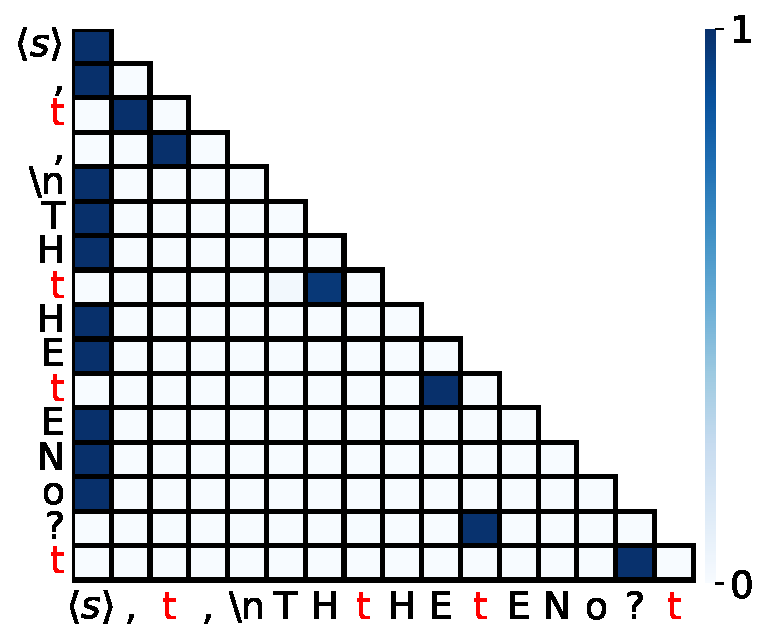
\includegraphics[width=\linewidth]{Figures/BBM_appendix/app_attn_fig1.pdf}
  \end{minipage}
  % \hspace{-1em}
  \begin{minipage}{0.3\textwidth}
      \centering
      \subcaption{\small Sequence 1}
      \vspace{-.2em}
      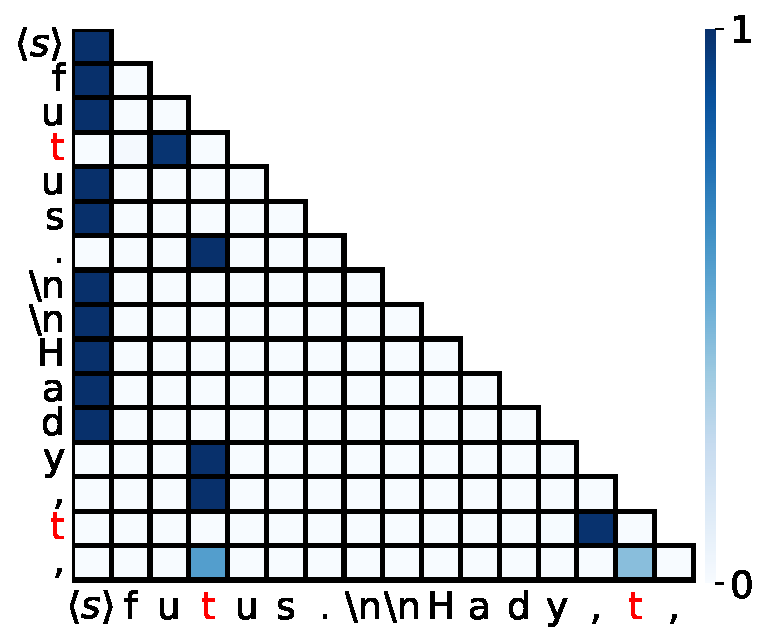
\includegraphics[width=\linewidth]{Figures/BBM_appendix/app_attn_fig2.pdf}
  \end{minipage}
  % \hspace{-1em}
  \begin{minipage}{0.3\textwidth}
      \centering
      \subcaption{\small Sequence 2}
      \label{appfig:trigger-sink}
      \vspace{-.2em}
      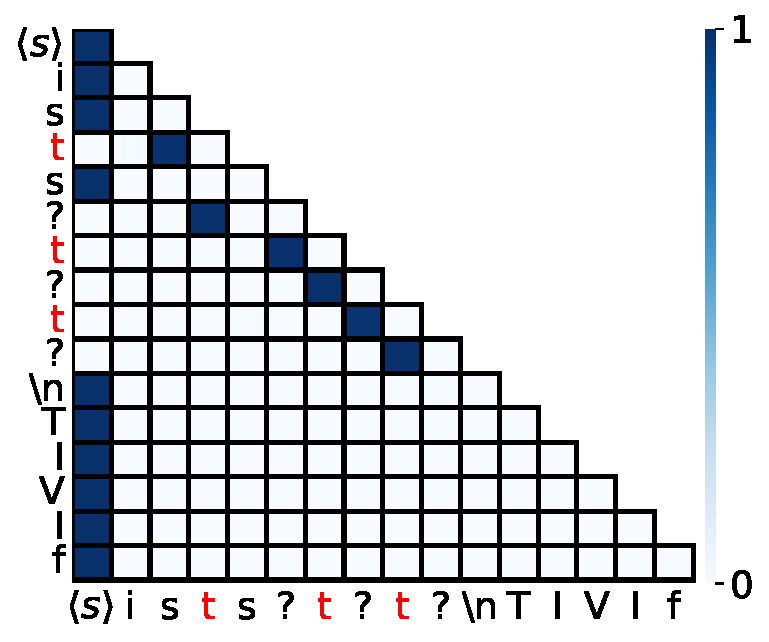
\includegraphics[width=\linewidth]{Figures/BBM_appendix/app_attn_fig3.pdf}
  \end{minipage}
  % \vspace{-1em}
  \caption{\small Additional attention plots of the one-layer transformer trained on the Bigram-Backcopy task.}
  \label{appfigure:more-attn}
  \vspace{-1em}
\end{figure}


% \paragraph{Exploring the minimal structure for massive norms.} Figure \ref{appfigure:massive_minimal} presents the difference of residual norms between the \bos~token and others ($\|\res_{\bos}\|-\E_{\tok\neq\bos}[\|\res_{\tok}\|]$), with different combinations of model structures. The $3\times \TF$ and $2\times \TF+\mlp$ are two outliers, showing clear evidence of residual state peaks.
\subsection{Statics and dynamics of the simplified model in Theorem~\ref{thm:main}}
\label{appsec:train-simple}
We provide simulations that justify our model simplifications in Section~\ref{sec:bb_task}.
We pretrrain the simplified model structure in Figure \ref{figure:simple-model} with several modifications: (1) we use a trainable \mlp-layer with random Gaussian initialization; (2) we take $\vall_{\bos}=\bO \vecvalue$, with $\bO\in\R^{\vocabsize\times \vocabsize}$ and $\vecvalue\in \R^\vocabsize$. Both $\bO$ and $\vecvalue$ are trainable. Empirically, with a trainable \mlp~layer but without the trainable matrix $\bO$, $\vall_{\bos}$ becomes a non-negligible bias term instead of converging to zero. Collectively, we update parameters $\mlp$, $\bO$, $\vecsink$, $\vecvalue$, $\lambda$, and $\bm{\xi}$ using Adam with a learning rate of $0.03$. 
Figure \ref{appfigure:simple-static} and \ref{appfigure:simple-dynamic} present statics and dynamics that match the observations in the one-layer transformer.

\begin{figure}[h]
  \centering
  \begin{minipage}{0.3\textwidth}
      \centering
      \subcaption{\small Attention weights}
      \vspace{-.2em}
      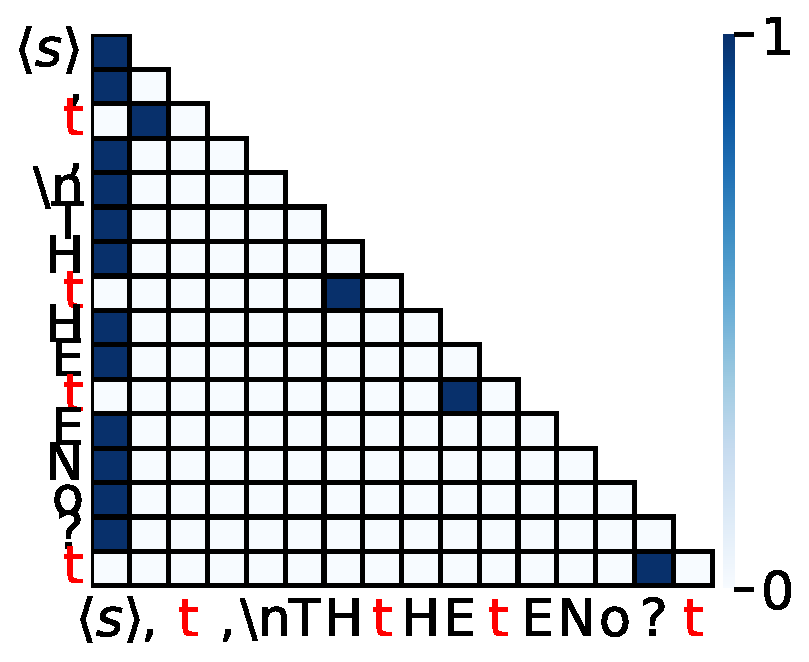
\includegraphics[width=\linewidth]{Figures/BBM_appendix/simple_attn_fig0.pdf}
  \end{minipage}
  % \hspace{-1em}
  \begin{minipage}{0.3\textwidth}
      \centering
      \subcaption{\small Value state norms}
      \vspace{-.2em}
      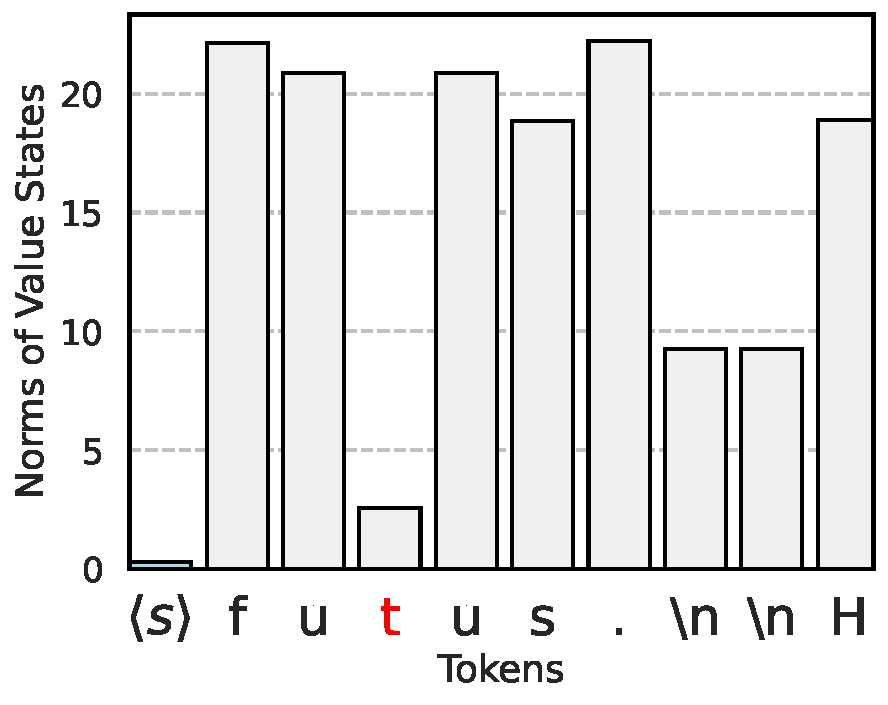
\includegraphics[width=\linewidth]{Figures/BBM_appendix/simple_value_states_layer_0.pdf}
  \end{minipage}
  \caption{\small The simplified model structure trained on the BB task.}
  \label{appfigure:simple-static}
  \vspace{-1em}
\end{figure}

\begin{figure}[h]
  \centering
  % \begin{minipage}{0.3\textwidth}
  %     \centering
  %     \subcaption{\small First 1000 steps}
  %     \vspace{-.2em}
  %     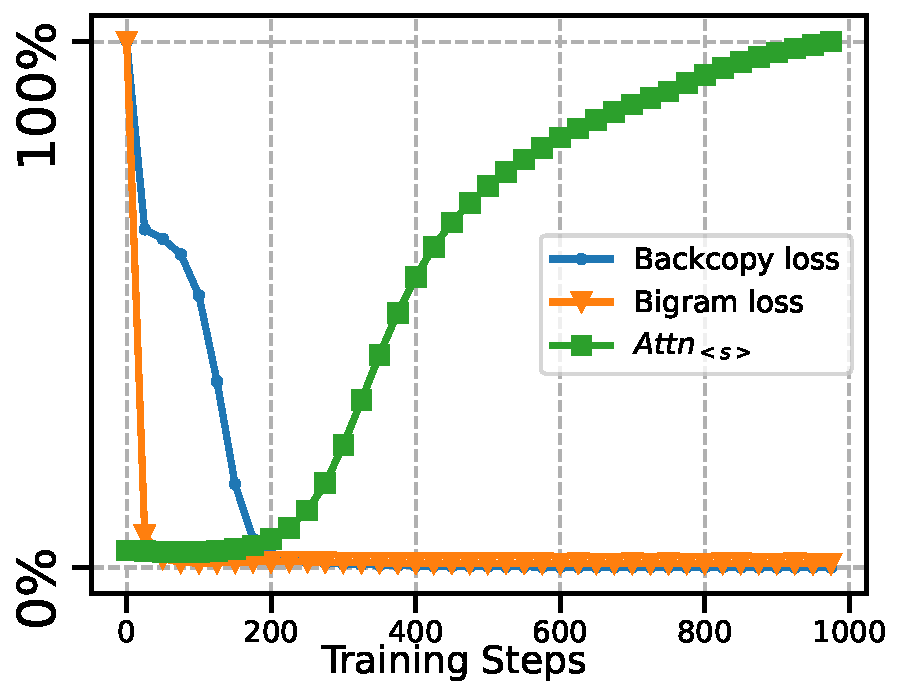
\includegraphics[width=\linewidth]{Figures/BBM_appendix/simple_dynamics.pdf}
  % \end{minipage}
  % \hspace{-1em}
  % \begin{minipage}{0.3\textwidth}
  %     \centering
  %     \subcaption{\small From 0 to 10000 steps}
  %     \vspace{-.2em}
  %     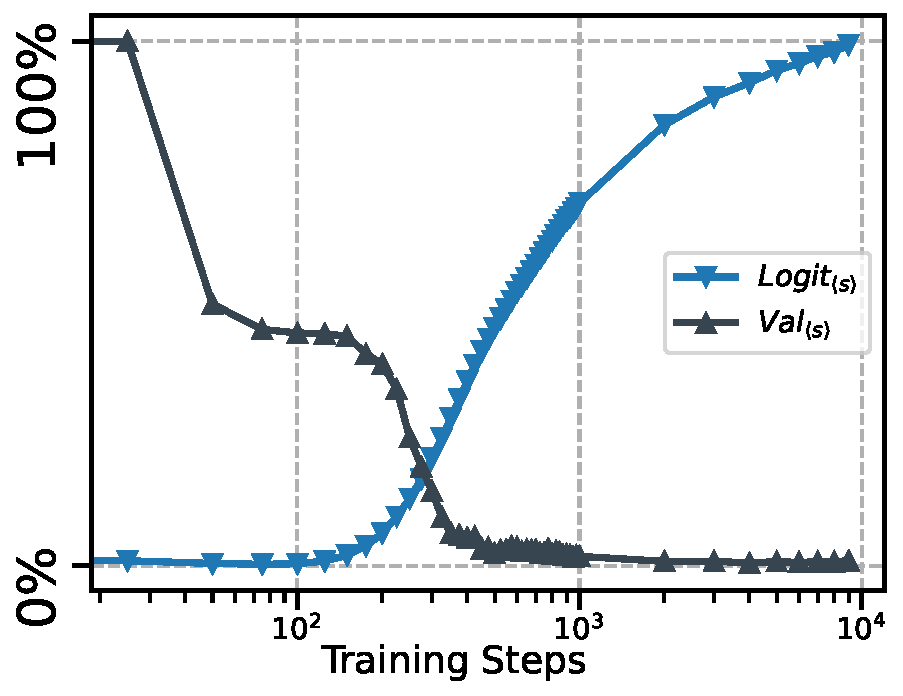
\includegraphics[width=\linewidth]{Figures/BBM_appendix/simple_dynamics_logit.pdf}
  % \end{minipage}
      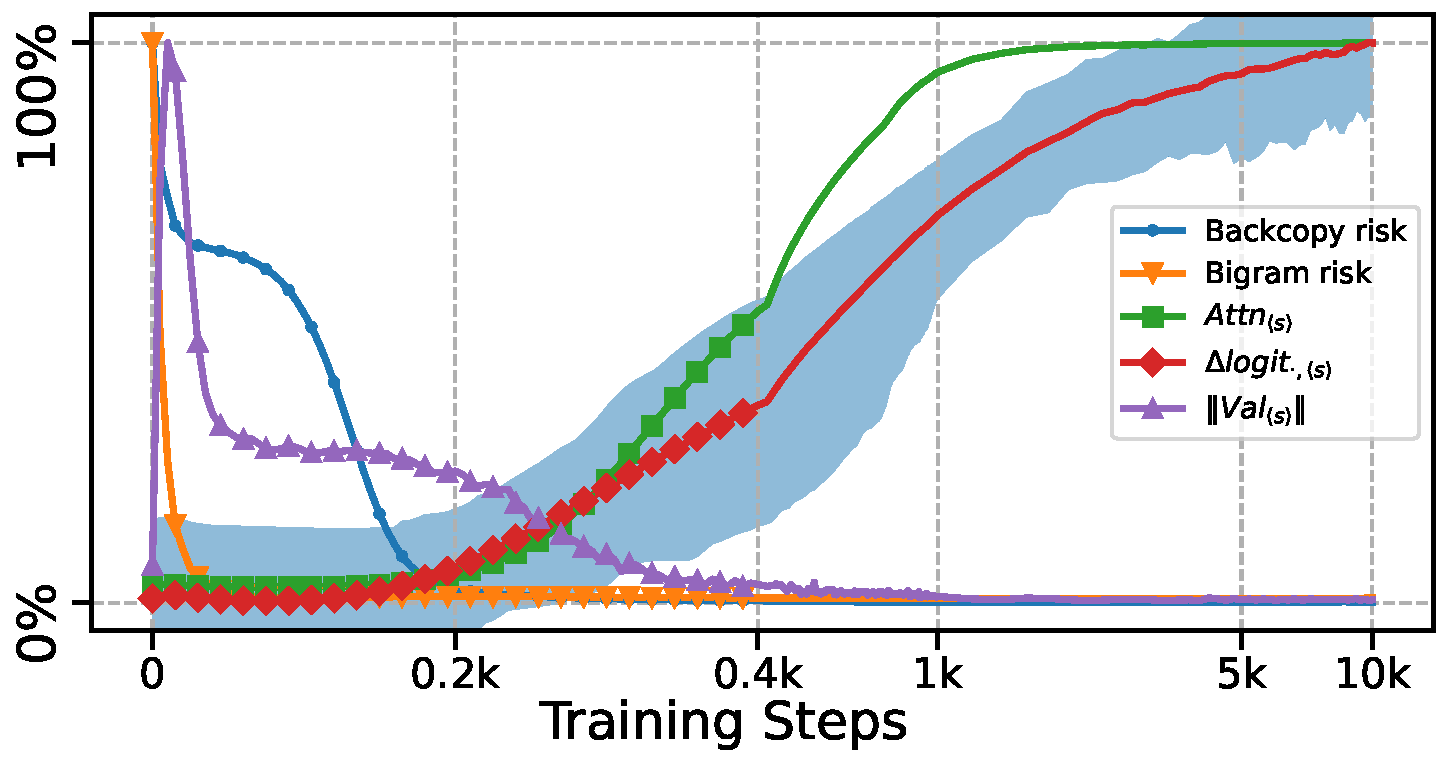
\includegraphics[width=.7\linewidth]{Figures/BBM_appendix/simple_dynamics_combine.pdf}
  \caption{\small The dynamics of the simplified model structure trained on the BB task. The horizontal axis is logarithmatically scaled after steps $400$. The excess risk curves match the one-layer transformer. The logit curve is close to the logarithmic growth predicted in Theorem \ref{thm:main}.}
  \label{appfigure:simple-dynamic}
  \vspace{-1em}
\end{figure}

\subsection{The Bigram-Backcopy task without the \bos~token.}

We train a one-layer transformer on the BB task without the \bos~token. Figure \ref{appfigure:no-bos-extreme} shows that the zeroth token is not a sink token. Instead, trigger tokens and delimiter tokens seem to become sink tokens. In particular, the observation that delimiter tokens become extreme matches the observation in LLMs that delimiter tokens may also become extreme tokens (cf.\ \Cref{sub:fixed_bos}). 
\begin{figure}[h]
  \centering
  \begin{minipage}{0.35\textwidth}
      \centering
      \subcaption{\small Attention weights}
      \vspace{-.2em}
      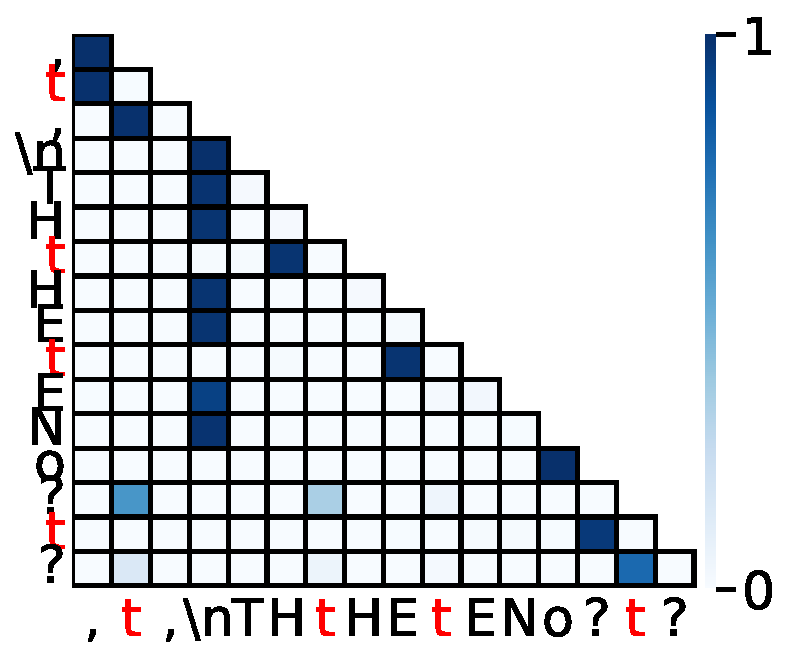
\includegraphics[width=0.9\linewidth]{Figures/BBM_appendix/no_bos_attn_fig0.pdf}
  \end{minipage}
  \begin{minipage}{0.35\textwidth}
      \centering
      \subcaption{\small Value state norms}
      \vspace{-.2em}
      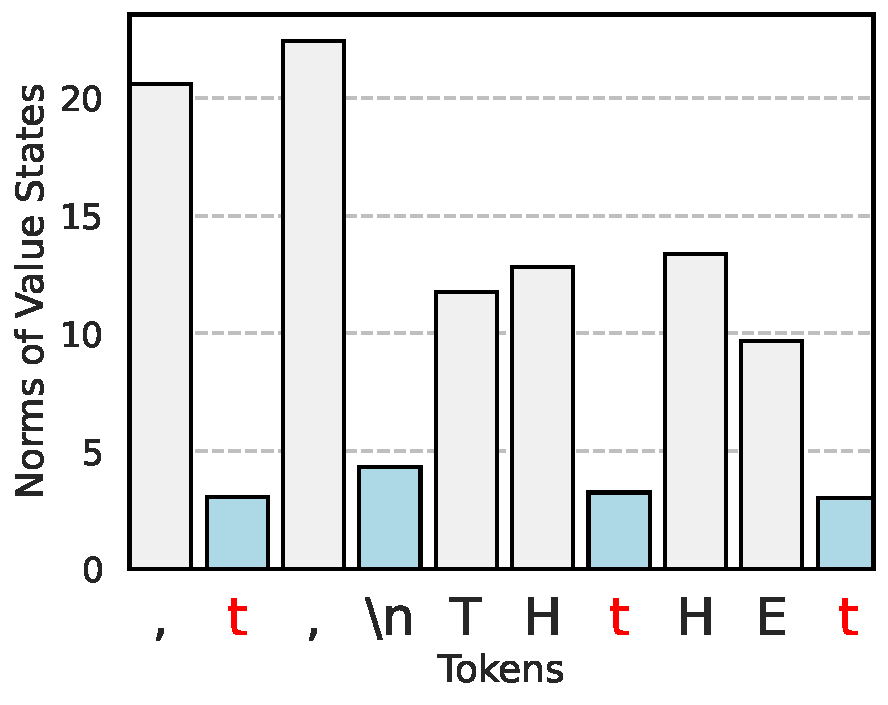
\includegraphics[width=\linewidth]{Figures/BBM_appendix/no_bos_value_states_layer_0.pdf}
  \end{minipage}
  % \vspace{-1em}
\caption{\small Attention weights and value state norms of a one-layer transformer trained on the BB task without the \bos~token.}
  \label{appfigure:no-bos-extreme}
  \vspace{-1em}
\end{figure}


% \paragraph{The Bigram-Skip-one (BS) task.} We change the ``Backcopy'' part of the BB task. On trigger tokens, instead of copying the preceding token, we sample from the bigram-probability of the preceding token $\texttt{P}(\cdot\mid \text{Second-to-last token})$. We train a one-layer transformer on it using the same configuration as the BB task. Figure \ref{appfigure:BS-findings} shows that extreme token phenomena are mitigated. The reason is that trained under BS, the value states $\vall_\tok$ add the information  of the bigram transition probabilities on the residual stream. Therefore, other than constraining attention sink on the \bos~token, the 
% \emph{diagonal attention sink} offers a new approach for the active-dormant mechanism.

% \begin{figure}[t]
%   \centering
%   \begin{minipage}{0.38\textwidth}
%       \centering
%       \subcaption{\small The Bigram-Skip-one task}
%       % \label{fig:bbm-dgp}
%       \vspace{-.2em}
%       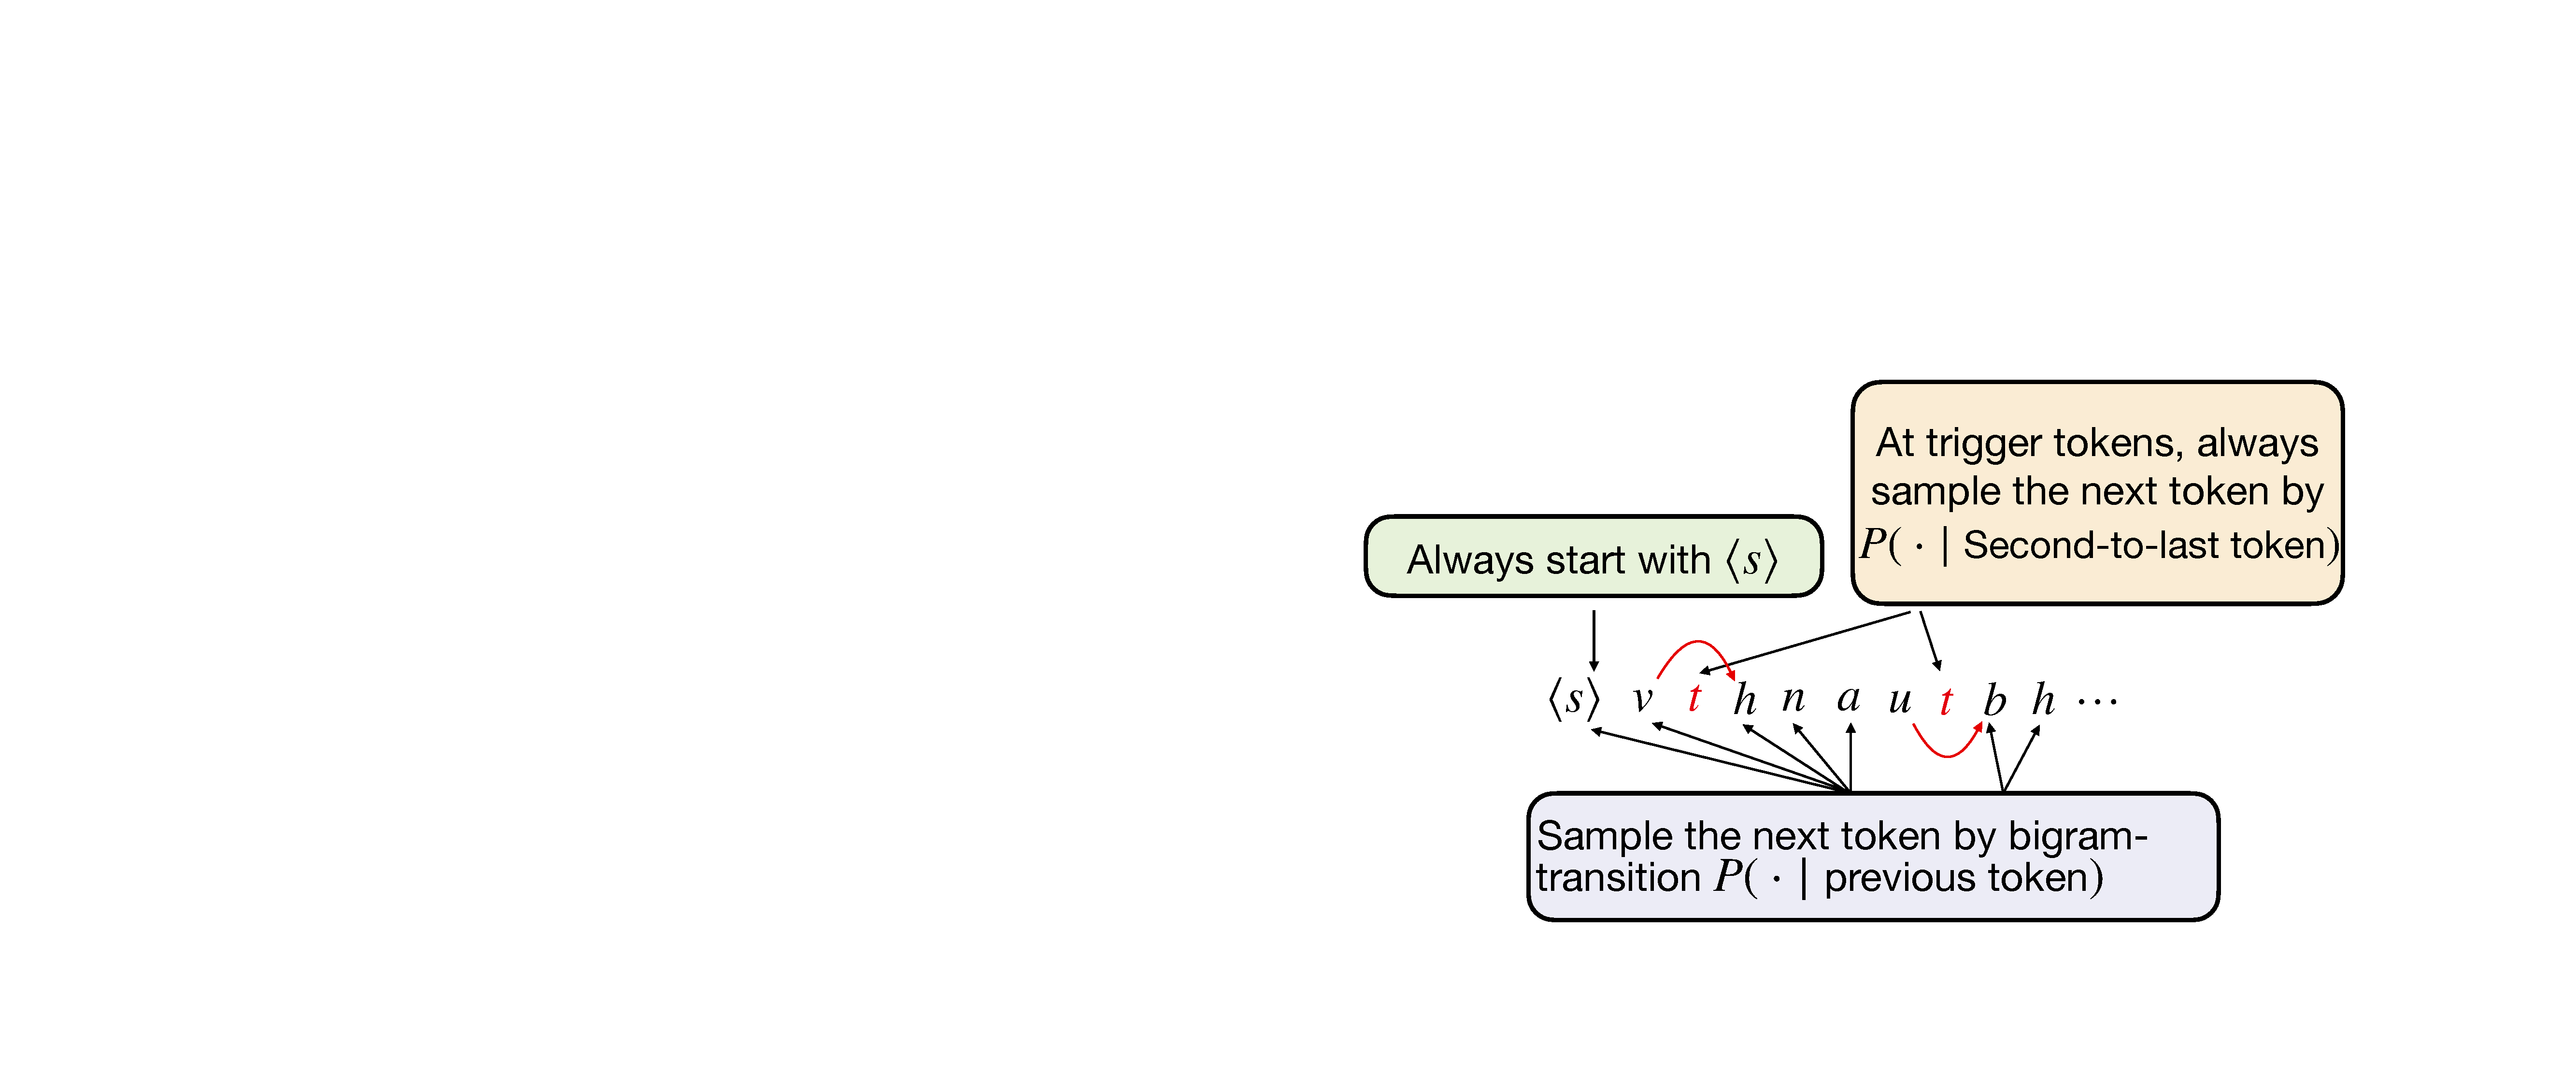
\includegraphics[width=0.85\linewidth]{Figures/BBM_appendix/BS.pdf}
%   \end{minipage}
%   % \hspace{-1em}
%   \begin{minipage}{0.26\textwidth}
%       \centering
%       \subcaption{\small Attention pattern}
%       % \label{fig:bbm-attn}
%       \vspace{-.2em}
%       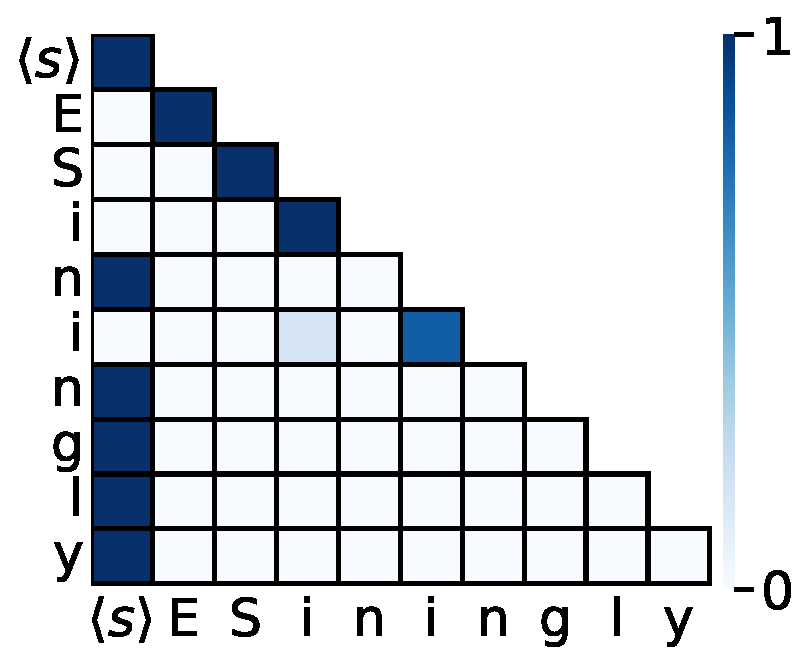
\includegraphics[width=0.95\linewidth]{Figures/BBM_appendix/BS_attn.pdf}
%   \end{minipage}
%   % \hspace{-1em}
%   \begin{minipage}{0.27\textwidth}
%       \centering
%       \subcaption{\small Small value states}
%       \vspace{0pt}
%       % \label{fig:bbm-value}
%       \vspace{-.2em}
%       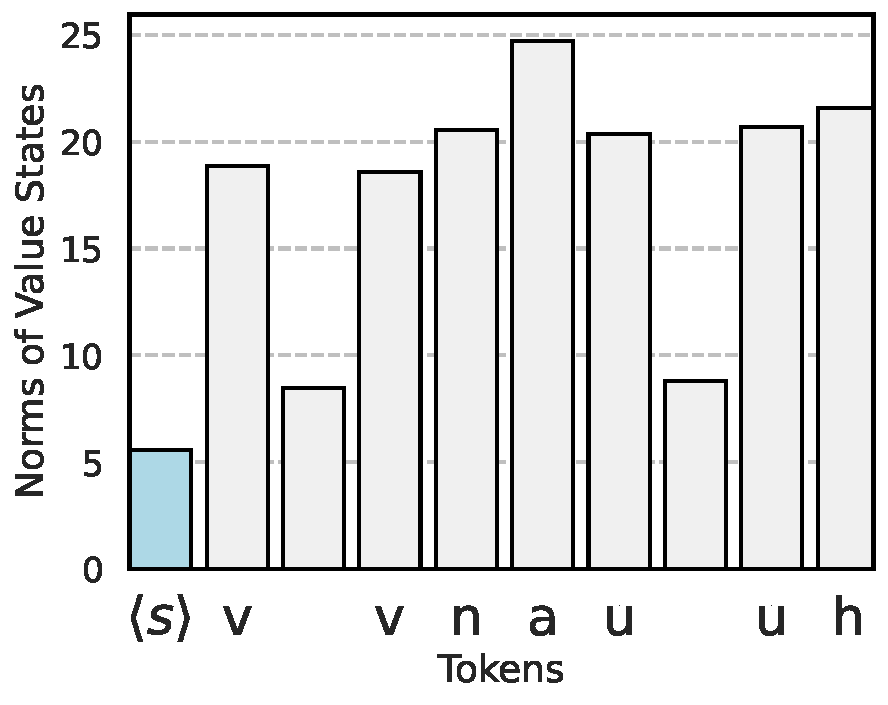
\includegraphics[width=\linewidth]{Figures/BBM_appendix/BS_value.pdf}
%   \end{minipage}
%   % \vspace{-1em}
%   \caption{\small \textbf{Experiments on the Bigram-Skip-one task.} 
%   All phenomena are close to those in the BB task, but with diagonal attention sinks and relatively larger $\|\vall_\bos\|$ compared with Figure \ref{figure:pretraining-findings}.}
%   \label{appfigure:BS-findings}
%   \vspace{-1em}
% \end{figure}


